\documentclass[a4paper,fleqn,12pt]{article}
\usepackage[utf8]{inputenc}
\usepackage{amsmath}
\usepackage{amssymb}
\usepackage{booktabs}
\usepackage{fancyhdr}
\usepackage{amsthm}
\usepackage{graphicx}
\usepackage{pdfpages}

\begin{document}
\begin{titlepage}
	\setlength{\parindent}{0pt}
	\large
\centering
Techincal University - Sofia \par
Faculty of Applied Mathematics and Informatics \par
\vspace{2cm}

{\huge Project 1 - Topics of Algebra\par}

\vspace{2cm}

\vspace{1cm}
{\LARGE\scshape  Solution for version 4 \par}



\vfill

\begin{minipage}[t]{.5\linewidth}
	Student: \\
	Kristian Krachmarov \\
	791324005
\end{minipage}%
\begin{minipage}[t]{.5\linewidth}
	\raggedleft
	Examiner:\\
	Prof. Mirko Tarulli
\end{minipage}

\vspace{2cm}
\raggedright

\end{titlepage}
\pagenumbering{gobble}
\tableofcontents
\newpage
%\fontsize{14pt}{16pt}\selectfont
\pagenumbering{arabic}
\newpage

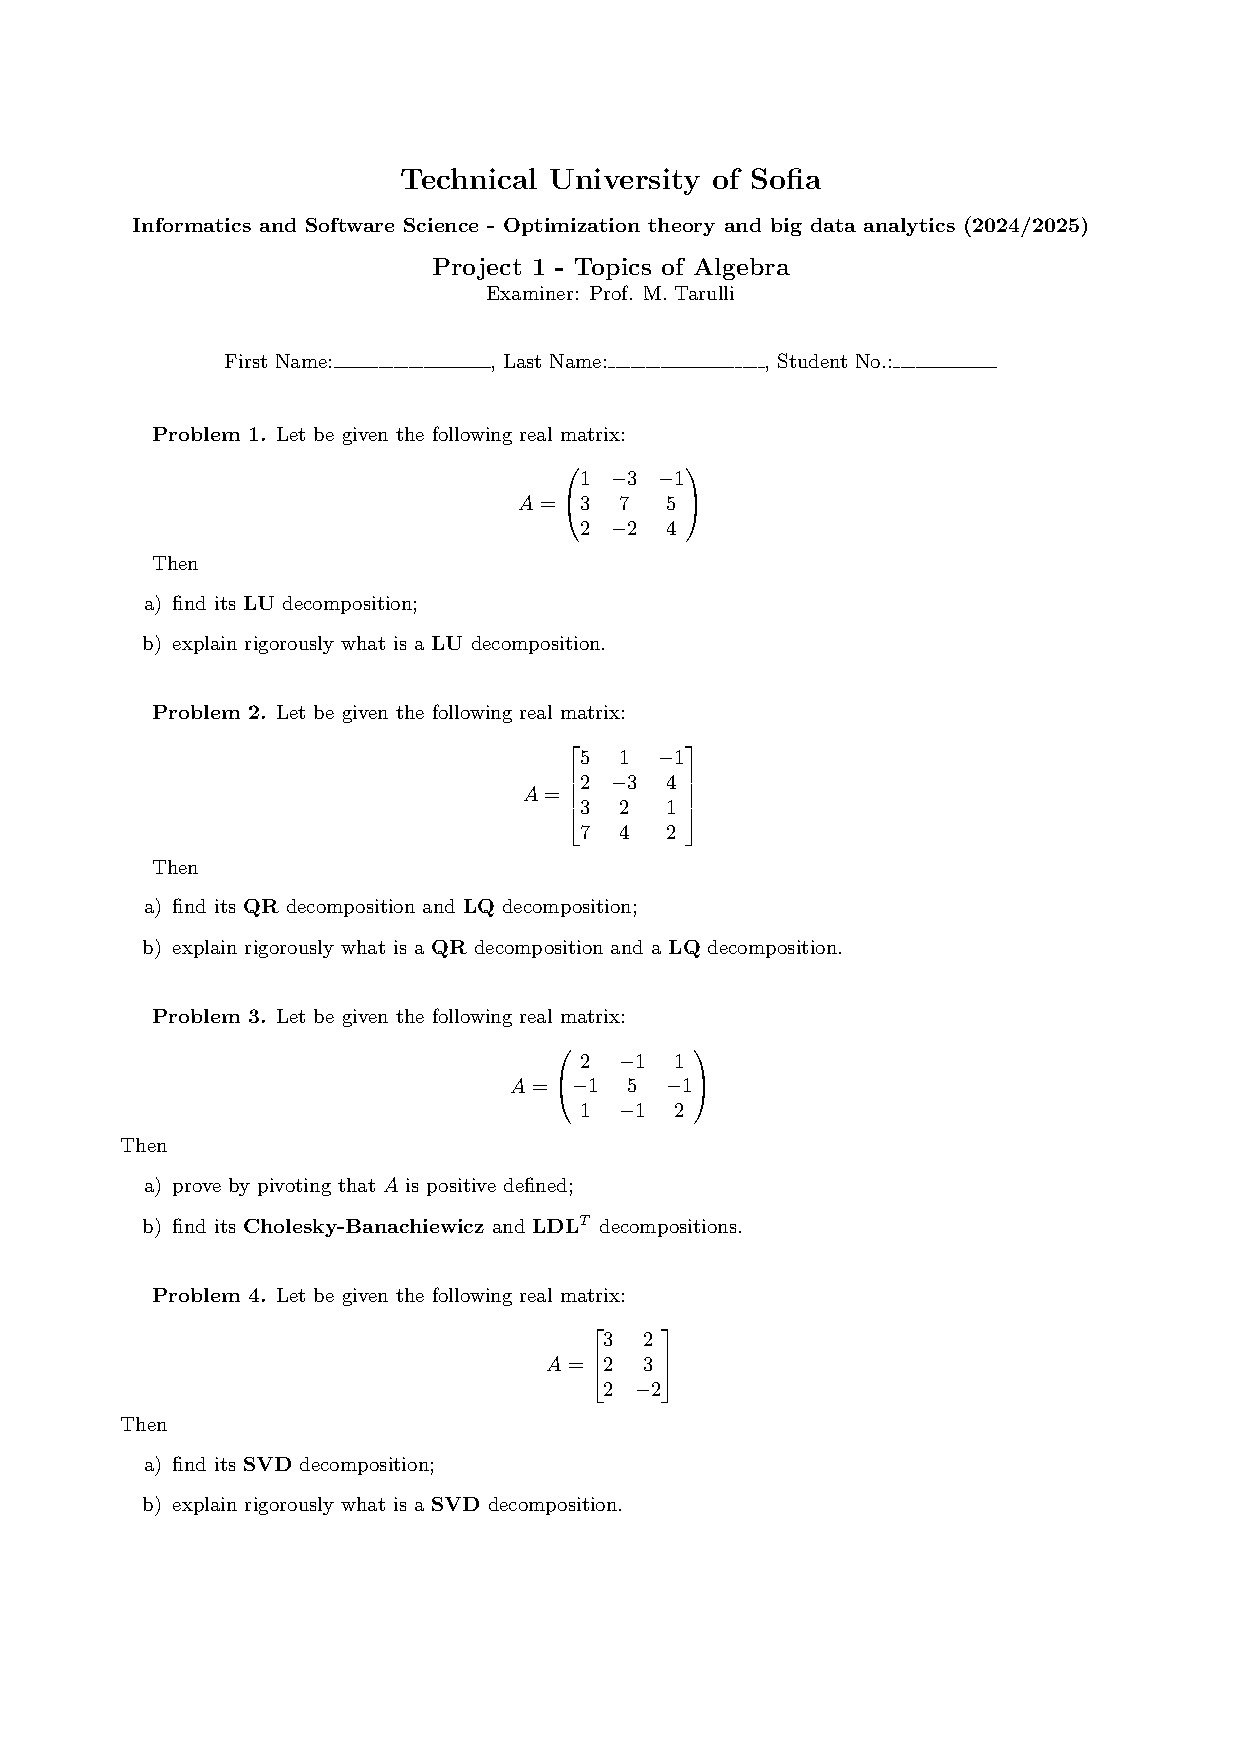
\includepdf[pages=-]{Project1-Version4-2425.pdf}
\newpage

\section{Problem 1}
$$ A = 
	\begin{pmatrix}
	1 & -3 & -1 \\
	3 & 7 & 5 \\
	2 & -2 & 4 \\
	\end{pmatrix}
$$
\subsection{Solution for 1a}
Lets start with L being the identity matrix
$$
	L = \begin{pmatrix}
	1 & 0 & 0 \\
	0 & 1 & 0 \\
	0 & 0 & 1 \\
	\end{pmatrix}
$$
We perform the following operations on matrix A: 
$$
\begin{array}{|l@{}}
	R_2 = R_2 - 3R_1 \\
	R_3 = R_3 - 2R_1
\end{array}
$$
Where $R_i$ is the $i$th row of the matrix. \\
We write the coefficient 3 in the matrix L at row 2 and column 1. 
The same can be done for the coefficient 2 for row 3 and column 1.
$$
	L = \begin{pmatrix}
	1 & 0 & 0 \\
	3 & 1 & 0 \\
	2 & 0 & 1 \\
	\end{pmatrix} \qquad 
	A = \begin{pmatrix}
	1 & -3 & -1 \\
	0 & 16 & 8 \\
	0 & 4  & 6 \\
	\end{pmatrix}
$$
We perform the following operation on matrix A
$$
R_3 = -\frac{1}{4}R_2 + R_3
$$
We write the coefficient $\frac{1}{4}$ in matrix L at row 3 and column 2.
$$
L = \begin{pmatrix}
	1 & 0 & 0 \\
	3 & 1 & 0 \\
	2 & \frac{1}{4} & 1 \\
	\end{pmatrix} \qquad 
	A = \begin{pmatrix}
	1 & -3 & -1 \\
	0 & 16 & 8 \\
	0 & 0  & 4 \\
	\end{pmatrix} = U
$$
\newpage
\subsection{Solution for 1b}

\newpage

\section{Problem 2}
$$
A = \begin{bmatrix}
	5 & 1 & -1 \\
	2 & -3 & 4 \\
	3 & 2 & 1 \\
	7 & 4 & 2 \\
\end{bmatrix}
$$
\subsection{Solution for 2a}
\subsection{Solution for 2b}
\newpage

\section{Problem 3}
\subsection{Solution for 3a}
\subsection{Solution for 3b}
\newpage

\section{Problem 4}
\subsection{Solution for 4a}
\subsection{Solution for 4b}


















































\end{document}